\documentclass{beamer}
% francification de LaTeX
\usepackage[utf8]{inputenc}
\usepackage[french]{babel}
% imagination
\usepackage{tikz}
% options de beamer
\usetheme{Boadilla}
\title{Projet \textit{Labyrinthe}}
\subtitle{Algorithmes et Structures de Donnée}
\author{Juan-Carlos Barros et Daniel Kessler}
% des compteurs pour l'importation d'images
\usepackage{forloop}
\newcounter{onlynumber}
\newcounter{pngnumber}
% code
\usepackage{listingsutf8}
\definecolor{lstcolor}{rgb}{0.9,0.95,0.95}
\definecolor{lstcommentcolor}{rgb}{0.,0.2,0.}
\lstset{
  frameround=tttt,
  %autogobble,
  frame=single,
  backgroundcolor=\color{lstcolor},
  % extendedchars=true,
  % basicstyle=\ttfamily\small,
  keywordstyle=\bfseries\color{blue},
  identifierstyle=\bfseries\color{red},
  stringstyle=\bfseries\color{orange},
  commentstyle=\color{lstcommentcolor},
  language=Python,
  keepspaces=True,
  basicstyle=\fontfamily{pcr}\selectfont\small, % monospace it for copypasting
  upquote=true,
  columns=flexible,
  showstringspaces=False,
  literate={é}{{\'e}}1
}
% et c'est parti
\begin{document}

\begin{frame}
  \titlepage
\end{frame}

\begin{frame}
%  \frametitle{}
  % Formation \textit{GymInf},
  Cours d'\textit{\textcolor<1>{blue}{Algorithmes}}
  et \textit{\textcolor<1>{green}{Structures de donnée}}
  \par\bigskip
  \onslide<2->{Projet \textit{Labyrinthe}}\par
  \begin{minipage}{.5\linewidth}
  \begin{itemize}
  \item<2->\textcolor{blue}{Algorithme}\par\onslide<3->{A*}
  \item<2->\textcolor{green}{Structure de Donnée}\par\onslide<4>{Priority Queue}
  \end{itemize}
  \end{minipage}
  \begin{minipage}{.3\linewidth}
  \onslide<2->{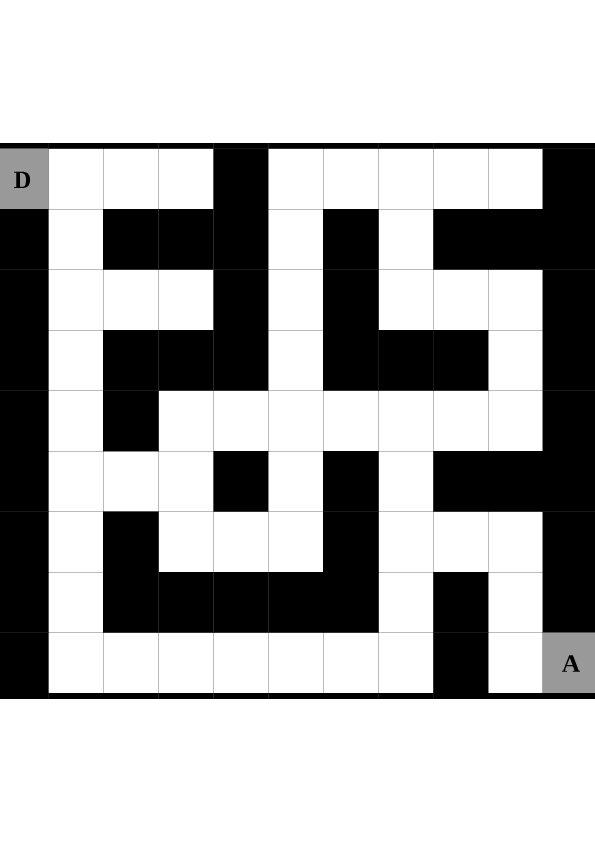
\includegraphics[width=\linewidth]{../diapos/V2bis/page1.png}}    
  \end{minipage}
\end{frame} % Titre

\begin{frame}
  \frametitle{Table des matières}
  \tableofcontents
\end{frame} % toc

\section{Quel algorithme pour résoudre quel problème?}
\subsection{Choix du problème}
\begin{frame} 
  \frametitle{Un labyrinthe, plusieurs problèmes}
  \begin{itemize}
  \item<1-> Cherche-t-on un chemin quelconque?
    \begin{itemize}
    \item<2-> Oui, on ne traversera le labyrinthe qu'une seule fois.
    \item<2-> \textbf<3->{Non, on veut le chemin le plus court}, pour peut-être le réutiliser.
    \end{itemize}
  \item<4-> Connait-on les coordonnées de la sortie dès le départ?
    \begin{itemize}
    \item<5-> \textbf<6->{Oui, et cette information pourra nous aider.}
    \item<5-> Non, le lieu de la sortie fait partie des inconnues.
    \end{itemize}
  \end{itemize}
\end{frame} % choix du problème

\subsection{Choix de l'Algorithme}
\begin{frame}
  \frametitle{Un problème, plusieurs solutions}
  \begin{itemize}
  \item<1-> Breadth-First Search
    \begin{itemize}
    \item garantit de trouver une solution si elle existe
    \item solution optimale si tous les pas sont égaux
    \end{itemize}
  \item<2-> Dijkstra
    \begin{itemize}
    \item choisit où explorer selon les distances déjà parcourues
    \item garantit de trouver le plus court chemin
    \end{itemize}    
  \item<3-> A*
    \begin{itemize}
    \item nécessite de connaître les coordonnées de la sortie
    \item choisit où explorer selon les distances déjà parcourues et la distance
      à la sortie
    \end{itemize}
  \end{itemize}
\end{frame}

\section{Algorithme A*}
\subsection{Pseudo-Code}
\begin{frame}
  \frametitle{Algorithme A*}
  \begin{block}{pseudo-code}
    Démarrer une file d'attente avec la cellule de départ $D$, une liste de
    prédécesseurs avec $\{D:Nil\}$ et une liste de coûts d'accès avec
    $\{D:0\}$.
    \medskip
    
    \onslide<2->{Tant que la file d'attente n'est pas vide,}
    \begin{itemize}
    \item<3-> extraire (pop) la cellule prioritaire $C$ de la file d'attente
    \item<4-> si $C$ est la cellule d'arrivée $A$, retourner le chemin qui y amène
          (via backtracking sur les prédecesseurs)
    \item<5-> sinon, pour chaque voisin $V$ de $C$ qui n'est pas déjà accessible
      à moindre coût
      \begin{itemize}
      \item<6-> mémoriser le prédecesseur de $V$ et le coût d'accès à $V$
      \item<7-> ajouter $V$ à la file d'attente
      \end{itemize}
    \end{itemize}    
  \end{block}
\end{frame}

\subsection{Heuristique et Priorité}
\begin{frame}
  \frametitle{Heuristique et Priorité}
  La priorité d'une cellule $C$ en attente est le coût estimé d'un chemin
  complet passant par cette cellule.
  \smallskip

  priorité = coût\_réel ($D \rightarrow C$) + coût\_estimé ($C\rightarrow S$)

  \medskip
  \onslide<2->{La distance restante depuis une cellule jusqu'à l'arrivée doit être estimée
  \textit{sans jamais la surestimer}.}
  \begin{itemize}
  \item<3->{La \textbf{distance de Manhattan} $|\Delta x| + |\Delta y|$
    est un bon estimateur si les mouvements permis sont horizontaux et verticaux.}
  \par
  \item<4>{Une \textbf{heuristique nulle} ramène A* à l'algorithme de Dijkstra
      (ou Breadth-First Search sur grille carrée).}
  \end{itemize}
\end{frame}

\subsection{Structure de données ``Priority Queue''}
\begin{frame}
  \frametitle{File d'attente: ``Priority Queue''}
  \begin{itemize}
  \item Structure permettant insertion avec priorité et ``pop'' rapide de
    l'élément prioritaire
  \item Implémentation en Python en tant que \textbf{binary heap} avec le module \textit{heapq}
  \item Dans cette implémentation, vérifier si vide en $O(1)$, insertion et
    ``pop'' en $O\left(\log(n)\right)$ où $n$ est le nombre d'objets en attente\footnote{cf. https://www.cs.princeton.edu/~wayne/kleinberg-tardos/pdf/BinomialHeaps.pdf}
  % \item Un élément est un tuple (heuristique, numéro, contenu), ainsi en cas
  %   d'heuristique égale, le numéro le plus bas (insertion plus ancienne) donne
  %   la priorité
  \end{itemize}
\end{frame}
% \begin{frame}
%   \frametitle{Priority Queue pour A*}
%   \begin{itemize}
%   \item<1-> La priorité d'un noeud est le \textbf{coût heuristique} pour aller de
%     l'entrée à la sortie en passant par ce noeud.
%   \item<2-> Un élément de la queue a comme attributs l'identité du noeud, le
%     \textbf{coût réel} pour y accéder et son prédecesseur
%   \item<3-> La queue est initialisée avec le noeud de départ et un coût nul.
%   \end{itemize}
% \end{frame}

\subsection{Idée de preuve}
\begin{frame}
  \frametitle{Preuve de l'algorithme (grandes lignes)}
  L'heuristique $h(C)$ qui estime le chemin restant depuis une cellule $C$
  doit satisfaire deux conditions.
  \begin{enumerate}
  \item<2-> \textbf{Monotonicité}: sorte d'inégalité triangulaire faible
    $h(C_1) \leq r(C_1,C_2) + h(C_2)$ où $C_1, C_2$ sont deux cellules,
    $r(C_1, C_2)$ est la distance réelle entre elles.
    \par\smallskip
    \onslide<2->{Cette propriété garantit de trouver la sortie, sans se ``perdre'' dans des
      boucles éventuelles.}
  \item<3-> \textbf{Admissibilité: l'heuristique ne surestime jamais une distance}
    \par\smallskip
    \onslide<4->{Cela garantit qu'il n'y a pas de chemin plus court que celui
      trouvé.}\par\smallskip
    \onslide<5->{Par contradiction:}\onslide<6->{ s'il y en avait un, il aurait
      été estimé correctement ou sous-estimé, et serait donc prioritaire par
      rapport à un chemin complet trop long, vu qu'\textbf{un chemin complet
      a une priorité calculée uniquement en coût réel.}}
  \end{enumerate}
\end{frame}

\subsection{Exemple de résolution}
\begin{frame}
  \frametitle{Exemple de résolution}
  \begin{minipage}{.4\textwidth}    
    \only<1>{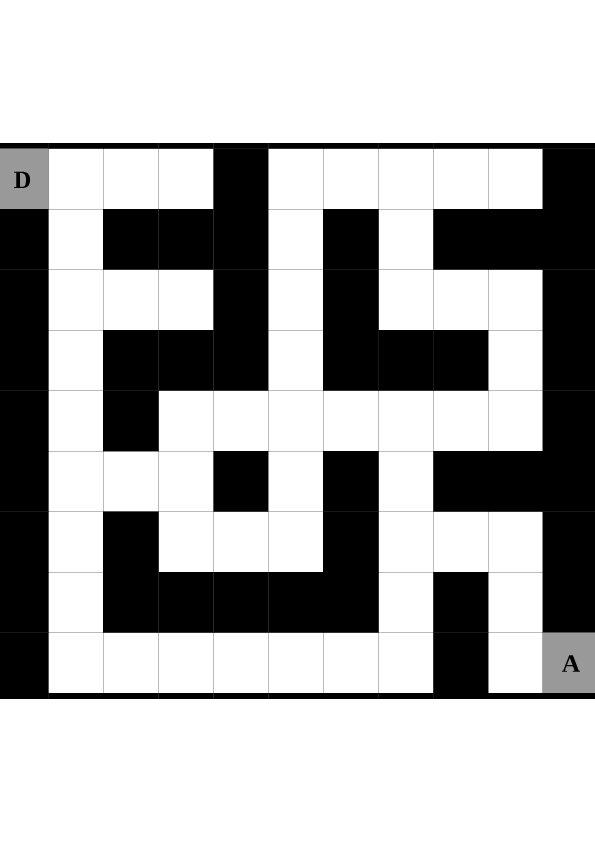
\includegraphics[width=\linewidth]{../diapos/V2bis/page1.png}}
    \only<2>{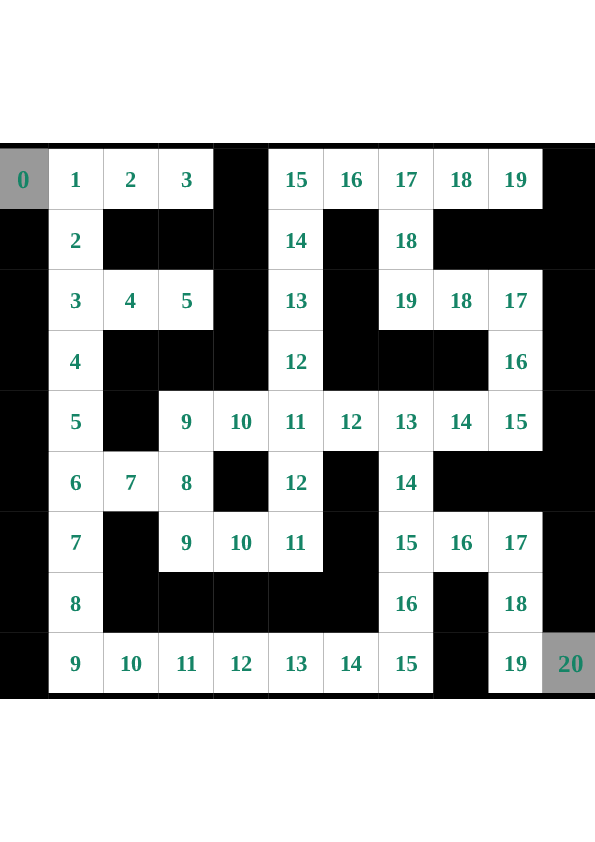
\includegraphics[width=\linewidth]{../diapos/V2bis/page2.png}} % 2 ou 4
    \only<3>{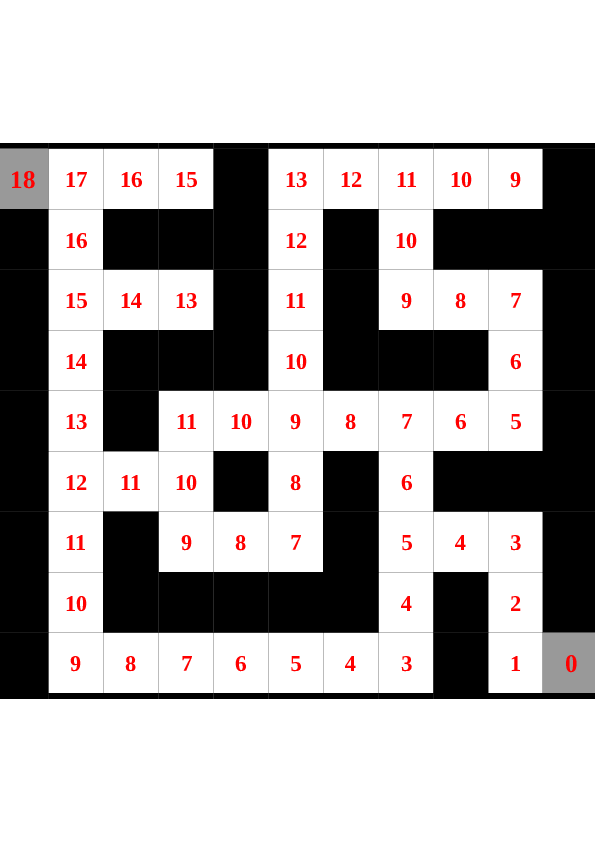
\includegraphics[width=\linewidth]{../diapos/V2bis/page5.png}} % 5 ou 6
    \only<4>{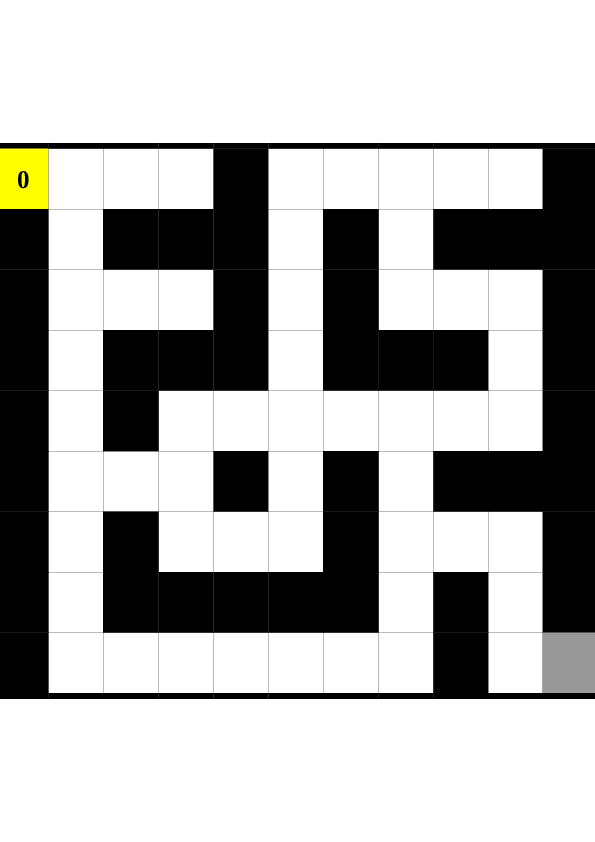
\includegraphics[width=\linewidth]{../diapos/V2/page1.png}}
    \setcounter{pngnumber}{2}
    \forloop{onlynumber}{5}{\value{onlynumber} < 66}{
      % \only<\arabic{onlynumber}>{only \theonlynumber, png \thepngnumber}\par
      \only<\arabic{onlynumber}>{\includegraphics[width=\linewidth]{../diapos/V2/page\arabic{pngnumber}.png}}
      \stepcounter{pngnumber}
    }
  \end{minipage}
  \quad
  \begin{minipage}{.55\textwidth}
    \only<1>{\textbf{Objectif}\par
      Trouver le chemin le plus court entre le \textbf{D}épart
      et l'\textbf{A}rrivée}
    \only<2>{Chaque noeud est à une distance réelle du départ, qui sera
      découverte en cours de route.}
    \only<3>{Chaque noeud est à une distance réelle de l'arrivée, mais ces
      distances ne sont pas encore connues.}
    \only<4>{Le départ est mis en file d'attente, avec une priorité 0.}
    \only<5>{Le seul voisin est évalué:
      \begin{itemize}
      \item coût réel pour y accéder: \textcolor{green}1
      \item coût heuristique pour la suite: \textcolor{red}{17}
      \item coût heuristique total (priorité): 18
      \end{itemize}
    }
    \only<6-43>{
      Légende:
      \begin{itemize}
      \item\textcolor{green}{coût réel jusqu'ici}
      \item\textcolor{red}{coût heuristique pour la suite}
      \item {coût heuristique total}
      \end{itemize}
      \medskip
      L'algorithme poursuit son chemin.}
    \par\medskip
    \only<7-8>{Parfois deux choix ont la même priorité, le choix est arbitraire.}
    \only<18-29>{Parfois la priorité participe vraiment au choix.}
    \only<34,38>{Parfois un nouveau chemin améliore l'accès à une même cellule.}
    \only<43->{Un chemin vers la sortie a été trouvé!}
    \onslide<44->{Backtracking pour reconstituer le chemin}
  \end{minipage}
\end{frame}

\section{Complexité}
\begin{frame}
  \frametitle{Complexité}
  Le pire des cas sera réalisé par un labyrinthe dont le meilleur chemin revient
  souvent en arrière (s'éloigne de l'arrivée). Dans ce cas, aucun gain n'est
  réalisé par rapport à l'algorithme de Dijsktra (ou ``heuristique nulle'').
  \par\medskip
  \onslide<2->{
  Dans ce cas, on aura visité toutes les $N$ cellules. Les coûts de
  lecture/écriture dans la file d'attente sont en $O(\log(n))$ où $n$ est le
  nombre d'éléments dans la ``frontière'' d'exploration, donc $n\sim O(\sqrt{N})$.
  Les autres opérations sont à coût comparable ou moindre. L'ensemble de la
  recherche sera donc en $O(N\log(N))$.}
  \par\medskip
  \onslide<3->{
  Cependant, le ``worst case'' ne rend pas justice à A* dont le but est
  justement d'éviter la plupart du temps le ``worst case'' avec un bon choix
  d'heuristique.
  }
\end{frame}

\section{Tests avec Python}
\defverbatim[colored]\code{
   marge = QueuePrioritaire(grid.start)\\
   cout\_reel = \{grid.start: 0\}\\
   parent = \{grid.start: None\}\\
\par\par
    while True:
        noeud\_courant = marge.pop()
        if noeud\_courant is None:
            raise ValueError("A*: la grille fournie n'a pas de solution")
        if noeud\_courant == grid.out:
            break  \# on a trouvé un chemin optimal vers la sortie
        for direction in ((0, 1), (1, 0), (0, -1), (-1, 0)):
            \# calculer coordonnées d'un voisin potentiel
            voisin = tuple([noeud\_courant[i] + direction[i] for i in (0, 1)])
            if voisin not in grid:
                continue  \# on ne peut pas accéder à ces coordonnées
            cout\_voisin = cout\_reel[noeud\_courant] + 1
            if voisin in cout\_reel and cout\_voisin >= cout\_reel[voisin]:
                continue  \# on a un meilleur chemin pour arriver à ce voisin
            \# on est arrivé jusqu'ici: ajouter le voisin à la marge
            cout\_reel[voisin] = cout\_voisin
            parent[voisin] = noeud\_courant
            marge.insert(cout\_voisin + distance(voisin, grid.out), voisin)
}
\begin{frame}[fragile]
  \frametitle{Tests avec Python}
  \begin{lstlisting}
marge = QueuePrioritaire(grid.start)
cout_reel = {grid.start: 0}
parent = {grid.start: None}

while True:
    noeud_courant = marge.pop()
    if noeud_courant is None:
        raise ValueError("la grille n'a pas de solution")
    if noeud_courant == grid.out:
        break  # chemin optimal trouvé
    # ... traiter noeud courant
\end{lstlisting}
la suite dans: \url{https://github.com/Dalker/ASD_labyrinthe/}
\end{frame}
\begin{frame}
  \frametitle{Tests avec Python}
  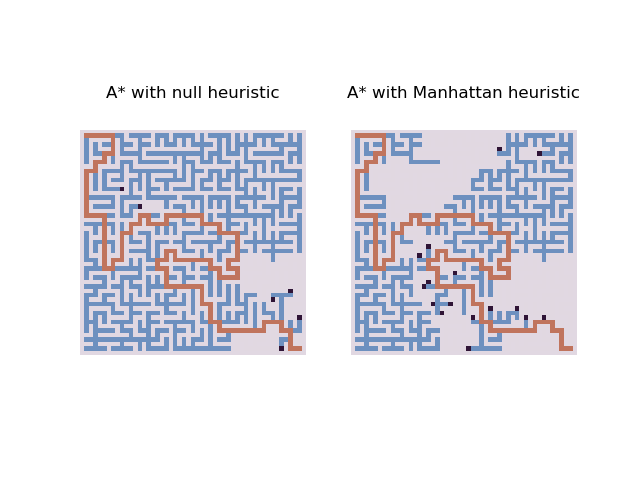
\includegraphics[width=.9\linewidth]{manhattan_vs_null.png}
\end{frame}

\begin{frame}
  \frametitle{Tests avec Python}
  \begin{semiverbatim}
    * Comparaison heuristique nulle vs Manhattan distance *
    
    solveur1 = heuristique 0, solveur2 = heuristique Manhattan
    
    30x30  : generate=0.1019s solve1=0.0060s solve2=0.0022s
    
    40x40  : generate=0.1814s solve1=0.0096s solve2=0.0086s
    
    50x50  : generate=0.5002s solve1=0.0228s solve2=0.0204s
    
    60x60  : generate=0.8701s solve1=0.0280s solve2=0.0199s
    
    70x70  : generate=1.0461s solve1=0.0451s solve2=0.0391s
    
    80x80  : generate=1.4218s solve1=0.0563s solve2=0.0423s
  \end{semiverbatim}
\end{frame}

\section{Conclusion}
\begin{frame}
  \frametitle{Conclusion}
  \begin{itemize}
  \item \ldots
  \item Robot-Aspirateur
  \end{itemize}
\end{frame}

\section{Références}
\begin{frame}
  \frametitle{Références}
  \begin{itemize}
  \item Liste des sources consultées:
    \url{https://github.com/Dalker/ASD_labyrinthe/wiki/Sources}
  \item Notre implémentation en Python, avec tests temporels et ``tests
    visuels'' (animations):
    
    \url{https://github.com/Dalker/ASD_labyrinthe/tree/main/implementation}
  \end{itemize}
\end{frame}
\end{document}